%!TEX root = draft.tex
\section{Modeling Network Structure}
\label{sec:Experiments}
In this section, we evaluate the effectiveness of our model in preserving
structural properties of six real-world networks described in \cref{sec:Datasets}.
Our experiments compare \texttt{ARW} to eight well-known growth models.
In~\Cref{sub:Experimental Setup}, we describe existing growth models and the evaluation metrics
used in the experiments. In~\Cref{sub:Experimental Results} , we discuss our
experimental results.

\subsection{Experiment Setup}
\label{sub:Experimental Setup}

% We first briefly summarize the existing models used in the experiments.
In this subsection, we describe the evaluation metrics used to quantify the extent to
which the following growth models preserve global structural properties of real-world networks.

\textit{Existing Growth Models}. We compare \texttt{ARW} to eight well-known
growth models that are representative of the key edge formation
mechanisms; Two of the eight models account for attribute homophily
and preserve attribute mixing patterns.
%  We consider two preferential attachment models, two attributed
% network growth models and two random walk models:

\begin{enumerate}
    \item{\textbf{Dorogovtsev-Mendes-Samukhin model}} \cite{dorogovtsev2000structure}  (\texttt{DMS})
    is a preferential attachment model in which the probability of linking to a node is proportional
    to the sum of its indegree and ``initial attractiveness.''

    \item{\textbf{Kim-Altmann model}} \cite{kim2017effect} (\texttt{KA}) is a fitness-based model that defines
    fitness as the product of degree and attribute similarity. It can generate \textit{attributed} networks with assortative mixing and
    heavy tailed degree distribution.

    \item{\textbf{Relay Linking model}} \cite{singh2017relay} (\texttt{RL}) propose a set of
    preferential attachment models that use relay linking to explain the change in node popularity over time.
    \footnote{We use the iterated preferential relay-cite (IPRC) variant, which best fits real-world network properties}

    \item{\textbf{Holme-Kim model}} \cite{holme2002growing} (\texttt{HK}) is a preferential attachment model
    which uses a triangle-closing mechanism to generate scale-free, clustered networks.

    \item{\textbf{Social Attribute Network model}} \cite{gong2012evolution} (\texttt{SAN}) generates
    scale-free, attributed networks with high clustering using attribute-augmented
    preferential attachment and triangle closing mechanisms.

    % We modify the model
    % to create directed edges and thereby generate directed networks.

    \item{\textbf{Herera-Zufiria model}} \cite{saramaki2004scale} (\texttt{SK})  is a random walk model
    that tunes the length of random walks to generate clustered networks with power law degree distributions.

    \item{\textbf{Saramaki-Kaski}} \cite{herrera2011generating} (\texttt{HZ}) is a random walk model
    that generates scale-free networks with tunable average local clustering.

    \item{\textbf{Forest Fire model}} \cite{leskovec2005graphs} (\texttt{FF}) is a recursive random walk model
    that preserves decreasing diameter over time, heavy-tailed degree distribution
    and high clustering.
\end{enumerate}

To ensure a fair comparison, we modify these models in three ways. First,
models that do not have an explicitly defined initial graph use the
initialization method described in~\Cref{sub:Model Fitting}. Second, we extend
models that use constant node outdegree by increasing outdegree over time
using the method described in \Cref{sub:Model Fitting}. Third, we adjust models
that generate undirected networks to create directed edges and thereby
generated directed networks.

\textit{Evaluation}. A network model fit should generate a network $\hat{G}$ that
preserves the global network structure of the observed network $G$. We evaluate
the fit by comparing four key global network properties of ${G}$ and $\hat{G}$:
degree distribution, local clustering distribution, degree-clustering relationship
and attribute assortativity.
We use the Kolmogorov-Smirnov (\texttt{KS}) statistic to compare the univariate degree
\& local clustering distributions.
% We use absolute difference to compare the
% attribute assortativity coefficients of networks $G$ and $\hat{G}$.
We compare the bivariate degree-clustering relationship in $G$ and $\hat{G}$ using
Weighted Relative Error (\texttt{WRE}). The evaluation metric \texttt{WRE} aggregates the relative error
between the average local clustering $c(k)$ and $\hat{c}(k)$ of nodes  with indegree $k$
in $G$ and $\hat{G}$ respectively; The weight of each relative error term equals the fraction
of nodes with indegree $k$ in $G$.

Jointly preserving multiple structural properties is a multi-objective optimization
problem; Model parameters that accurately preserve the degree distribution
(i.e. low \texttt{KS}) may not preserve the clustering distribution.
Therefore, we use grid search to select the model parameters that minimize the
$\ell^2$-norm of the aforementioned evaluation metrics. Since the evaluation metrics have
different scales, we normalize the metrics before computing the $\ell^2$-norm
to prevent any bias towards a particular metric.
We note that the sensitivity of the Forest Fire (\texttt{FF}) model necessitates a
manually guided grid search method.

% Next, we evaluate the performance of \texttt{ARW} in preserving multiple structural
% properties of six network datasets, relative to well-known existing models outlined
% in this subsection.

\begin{figure*}[t]
    \centering
    \vspace{-15mm}
    \makebox[\textwidth][c]{\includegraphics[width=\textwidth]{experiments_final2}}
    \vspace{-5mm}
    \caption{
    Modeling network structure. We assess the extent to which network models
    fit key structural properties of six real-world networks. Tables A, B and C
    measure the accuracy of eight models in fitting the indegree distribution,
    local clustering distribution, indegree-clustering relationship
    respectively and global attribute assortativity.
    %  Models with green \checkmark fit the assortativity
    % coefficient of attributed networks ---\texttt{ACL}, \texttt{APS} and
    % \texttt{Patents}--- up to 2 decimal places.
    % % We group models based on their
    % underlying edge formation mechanisms: preferential attachment, triangle closing
    % or random walks.
    Existing models tend to underperform because they either disregard
    the effect of factors such as triadic closure and/or homophily
    or are unable to generate networks with varying structural properties.
    Our model, \texttt{ARW}, jointly preserves all three properties accurately and often
    performs considerably better than existing models:
    The cells are shaded gray or dark gray if the proposed model \texttt{ARW} performs
    better at significance level $\alpha=0.01$ ( \lightgraybg{ }) or $\alpha=0.001$ ( \darkgraybg{ })
    respectively.
    % properties based on clustering. Models equipped with triangle closing
    % mechanisms ---\texttt{HK}, \texttt{SAN}---are not flexible enough to
    % accurately fit the skewed local clustering distributions of real-world
    % networks. Existing random walk models \texttt{FF}, \texttt{SK} and
    % \texttt{HZ} perform poorly because they are not expressive enough to
    % generate networks with varying structural properties.
    }
    \label{fig:exp_table}
\end{figure*}

\subsection{Experiment Results}
\label{sub:Experimental Results}

Our experiment results test the efficacy of \texttt{ARW} in \textit{jointly}
modeling multiple structural properties relative to well-known models outlined in
\cref{sub:Experimental Setup}. We evaluate the network models on network
datasets outlined in \cref{sec:Datasets}.

To evaluate the performance of network models, we first fit every model
to each network dataset $G$. Then, we compare the structural properties of
network dataset $G$ and network $\hat{G}$ generated by the fitted model using
metrics outlined in \cref{sub:Experimental Setup}. We evaluate multiple instances
of $\hat{G}$ to average out fluctuations and acquire data to conduct statistical tests.

Table \ref{fig:exp_table} lists the evaluation metrics for every pair of model
and dataset; The metrics measure the accuracy with which these models
preserve key global network properties: degree distribution, local clustering distribution
and indegree-clustering relationship.
We do not explicitly compare the extent to which these models preserve
attribute assortativity because the attribute related model parameters can be tuned to obtain
arbitrary precision. Instead, models that preserve assortativity up to two decimal
places --- \texttt{KA}, \texttt{SAN} and \texttt{ARW}
--- have green ticks (\checkmark) in table \ref{fig:exp_table}.
We use permutation testing to evaluate the relative performance of our model \texttt{ARW}. If
\texttt{ARW} performs better than a model on a dataset with significance level
$\alpha=0.01$ or $\alpha=0.001$, the corresponding cells in table \ref{fig:exp_table}
are shaded gray or dark gray boxes respectively.

% The performance of a model depends on the effectiveness of its underlying
% edge formation mechanisms. To study the strengths and weaknesses of these mechanisms,
% we group models (i.e. color-coded rows in table \ref{fig:exp_table}) based on their
% underlying edge formation mechanism: preferential attachment (blue), preferential attachment with
% triangle closing (orange) and random walk (green) mechanisms.

A common characteristic of existing models outlined in \cref{sub:Experimental Setup}
is that they fail to accurately preserve \textit{multiple} structural properties.
This is because existing models disregard important mechanisms such as triadic closure
\& homophily or are not flexible enough to generate networks with varying structural properties.

% For instance, the preferential attachment model \texttt{DMS}
% can accurately fit the heavy-tailed degree distributions but does not
% account for local clustering.
% On the other hand, the attributed network model \texttt{SAN} tries to preserve
% all four properties but cannot do so accurately.

Preferential attachment models \texttt{DMS}, \texttt{RL}
and \texttt{KA} preserve heavy tailed degree distributions but disregard
clustering. \texttt{DMS} outperforms other models in accurately modeling
degree distribution (table \ref{fig:exp_table}A) because its ``initial attractiveness''
parameter can be tuned to adjust preference towards low degree nodes. Unlike \texttt{KA}, however,
\texttt{DMS} cannot preserve global assortativity.
% \texttt{KA} outperforms \texttt{DMS} in preserving global assortativity because \texttt{KA}
% uses an attribute similarity parameter to model attribute mixing patterns.
By assuming that successive edge formations are independent, both models disregard
the effect of triadic closure and do not preserve local clustering. (tables \ref{fig:exp_table}B \& \ref{fig:exp_table}C).

\texttt{HK} and \texttt{SAN} are preferential attachment models
that use triangle closing mechanisms to generate networks with high average
local clustering and heavy tailed degree distributions.
Note that \texttt{HK} and \texttt{KA} fit degree distributions with the same \texttt{KS} statistic
(table \ref{fig:exp_table}A) because they lack parameters that can generate varying degree distributions.
While triangle closing leads to considerable improvement over \texttt{DMS}
and \texttt{KA} in modeling local clustering, \texttt{HK} and \texttt{SAN} are not flexibe enough
to preserve local clustering in \textit{all} datasets (see tables \ref{fig:exp_table}B \& \ref{fig:exp_table}C).
%  Nevertheless,
% barring one or two datasets in tables \ref{fig:exp_table}B and \ref{fig:exp_table}C,
% these models cannot accurately preserve the local clustering distribution and indegree-clustering
% relationship observed in real networks.

Existing random walk models \texttt{FF}, \texttt{SK} and \texttt{HZ}
are not flexible enough to accurately preserve network structure observed in real networks datasets.
The recursive approach in \texttt{FF}, wherein nodes perform a probabilistic breadth-first search
and link to \textit{all} visited nodes, considerably overestimates local clustering.
In \texttt{SK} and \texttt{HZ}, nodes perform a single random walk and link to
each visited node with some probability $\mu$; The parameter $\mu$ indirectly
controls the effect on triadic closure on edge formation
and leads to some improvement over \texttt{FF} in preserving local
clustering distribution (table \ref{fig:exp_table}B) and indegree-clustering relationship (table
\ref{fig:exp_table}). However, the improvements are not substantial when compared to the performance
of our model \texttt{ARW}. Furthermore, existing random walk models disregard attribute homophily
and do not model attribute mixing patterns.

The experiment results in table \ref{fig:exp_table} validate the effectiveness
of the proposed model \texttt{ARW} in \textit{jointly} preserving multiple
global network properties. \texttt{ARW} can generate networks with varying
degree distribution by adjusting nodes' preference towards high degree nodes
using out parameter $p_o$. As a result, \texttt{ARW} accurately preserves
degree distribution (table \ref{fig:exp_table}A), often significantly better
than all models except \texttt{DMS}. Similarly, \texttt{ARW} matches the local clustering
distribution  (table \ref{fig:exp_table}B) and indegree-clustering relationship
(table \ref{fig:exp_table}C) observed in real-world networks with high accuracy;
This is because the jump parameter $p_j$ and link parameter $p_l$ in \texttt{ARW}
control the effect of triadic closure on edge formation. Edge formation in \texttt{ARW}
depends on attribute similarity via attribute parameter $p_a$, which can be tuned to
match the attribute assortativity coefficient of attributed network datasets up to
arbitrary precision.
\begin{figure}
    \centering
    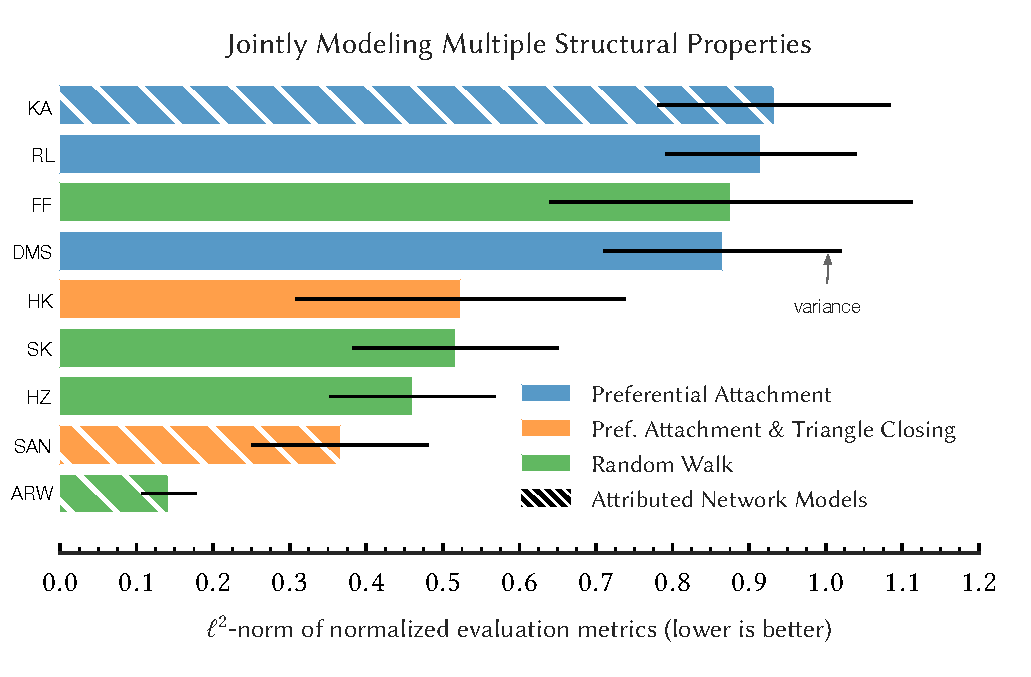
\includegraphics[width=.9\linewidth]{barplots_final3}
    \caption{Jointly modeling multiple network properties: \texttt{ARW} outperforms
    existing network models in jointly preserving key structural properties---indegree
    distribution, local clustering distribution and degree-clustering relationship---
    by a margin of 2.5-10x.
    % Unlike existing network models, \texttt{ARW} preserves multiple network
    % properties simultaneously because it unifies different sociological processes
    % into a single edge formation mechanism. Notably, \texttt{ARW} outperforms
    % existing network models by a margin of 2.5-10x.
     }
     \label{fig:barplot}
    % Existing network models perform poorly
    % because they make strong modeling assumptions that disregard individual resource constraints
    % and do not consider multiple factors that simultaneously influence edge formation.
\end{figure}

\Cref{fig:barplot} illustrates the performance of network models in jointly
modeling degree distribution, local clustering distribution and indegree-clustering
relationship. Preferential attachment models \texttt{KA}, \texttt{DMS} and
\texttt{RL} perform poorly because they do not preserve clustering. \texttt{HK}
and \texttt{SAN} perform better than \texttt{KA}, \texttt{DMS} and
\texttt{RL} because of edge formation mechanisms that close triangles
to preserve clustering and its relationship with degree to some extent. The proposed
model \texttt{ARW} outperforms existing random walk models \texttt{HZ}, \texttt{SK}
and \texttt{FF} by a considerable margin.  As shown in \cref{fig:barplot},
\texttt{ARW} improves upon the average $\ell^2$-norm of the second best performing model,
\texttt{SAN} by a margin of 2.5x.


% In \Cref{fig:barplot}, we show that \texttt{ARW} performs considerably better than
% six well-known, representative network models in jointly modeling
% degree distribution, local clustering distribution and indegree-clustering
% relationship.
% Preferential models \texttt{KA} and \texttt{DMS} perform poorly because
% they disregard clustering whereas the recursive approach in \texttt{FF} overestimates
% local clustering.
To summarize, \texttt{ARW} unifies multiple factors that influence edge formation
into a single mechanism. As a result, it can jointly preserve multiple structural
properties of real-world networks with high accuracy. Next, we discuss limitations
of the global assortativity coefficient and analyze local mixing pattterns of
real-world attributed networks.

\clearpage
\section{Modeling Local Mixing Patterns}
\label{subsec:LocalMixing}

The global assortativity coefficient quantifies
the level of homophily or heterophily in an attributed network. It sheds light
on the average propensity of links to occur between similar nodes by capturing
the attribute mixing pattern across the entire network.
However, global assortativity is not a representative summary statistic of heterogeneous mixing patterns
observed in large-scale networks. It does not quantify anomalous mixing patterns and
fails to measure how mixing varies across a network.

We use local assortativity \cite{peel2018multiscale} to measure varying
mixing patterns in an attributed network $G=(V,E,B)$ with attribute values $B=\{b_1...b_h\}$.
Unlike global assortativity that counts all edges between similar nodes, local assortativity of node $i$, $r_l(i)$,
captures mixing pattern in the local neighborhood of node $i$ by using a locality biased
weight distribution $w_i$; The distribution $w_i$ reweighs edges between similar nodes
based on how local they are to node $i$. Peel et al. \cite{peel2018multiscale} prescribe a
personalized pagerank weight distribution, which is prohibitively expensive to compute for
all nodes in large graphs; Large network datasets necessitate efficient weighting schemes.
Therefore, we define $w_i$ as a uniform distribution
over $N(i)$, the set of nodes that are at most 1 hop away from node $i$.
More formally, the local assortativity coefficient $r_l(i)$ of node $i$, with outdegree $m(i)$ and
attribute value $b(i)$ is defined as follows:
\vspace{-1mm}
\begin{align*}
    \scriptsize r_l(i) = \frac{\overbrace{\frac{1}{|N(i)|}\sum\limits_{j \in N(i)}^{m(j) > 0} \sum_{k \in V} \frac{\mathcal{I}\{(j,k) \in E \wedge b(j)=b(k)\}}{m(i)} }^{\texttt{obs}}-\overbrace{\sum_{b \in B} e_{b\cdot}e_{\cdot b}}^{\texttt{rnd}}}{\underbrace{1}_{\max(\texttt{obs})}-\underbrace{\sum_{b \in B} e_{b\cdot}e_{\cdot b}}_\texttt{rnd}}
\end{align*}
Intuitively, $r_l(i)$ compares the observed fraction of edges between similar nodes
in the local neighborhood of node $i$ (\texttt{obs}) to the expected fraction
if the edges are randomly rewired (\texttt{rnd}).

The local assortativity distributions
of \texttt{ACL}, \texttt{APS} and \texttt{Patents} reveal anomalous, skewed
and heterophilic local mixing patterns that are not easily inferred via the global assortativity,
as shown in \cref{fig:local_atty}.
\begin{figure}
    \centering
    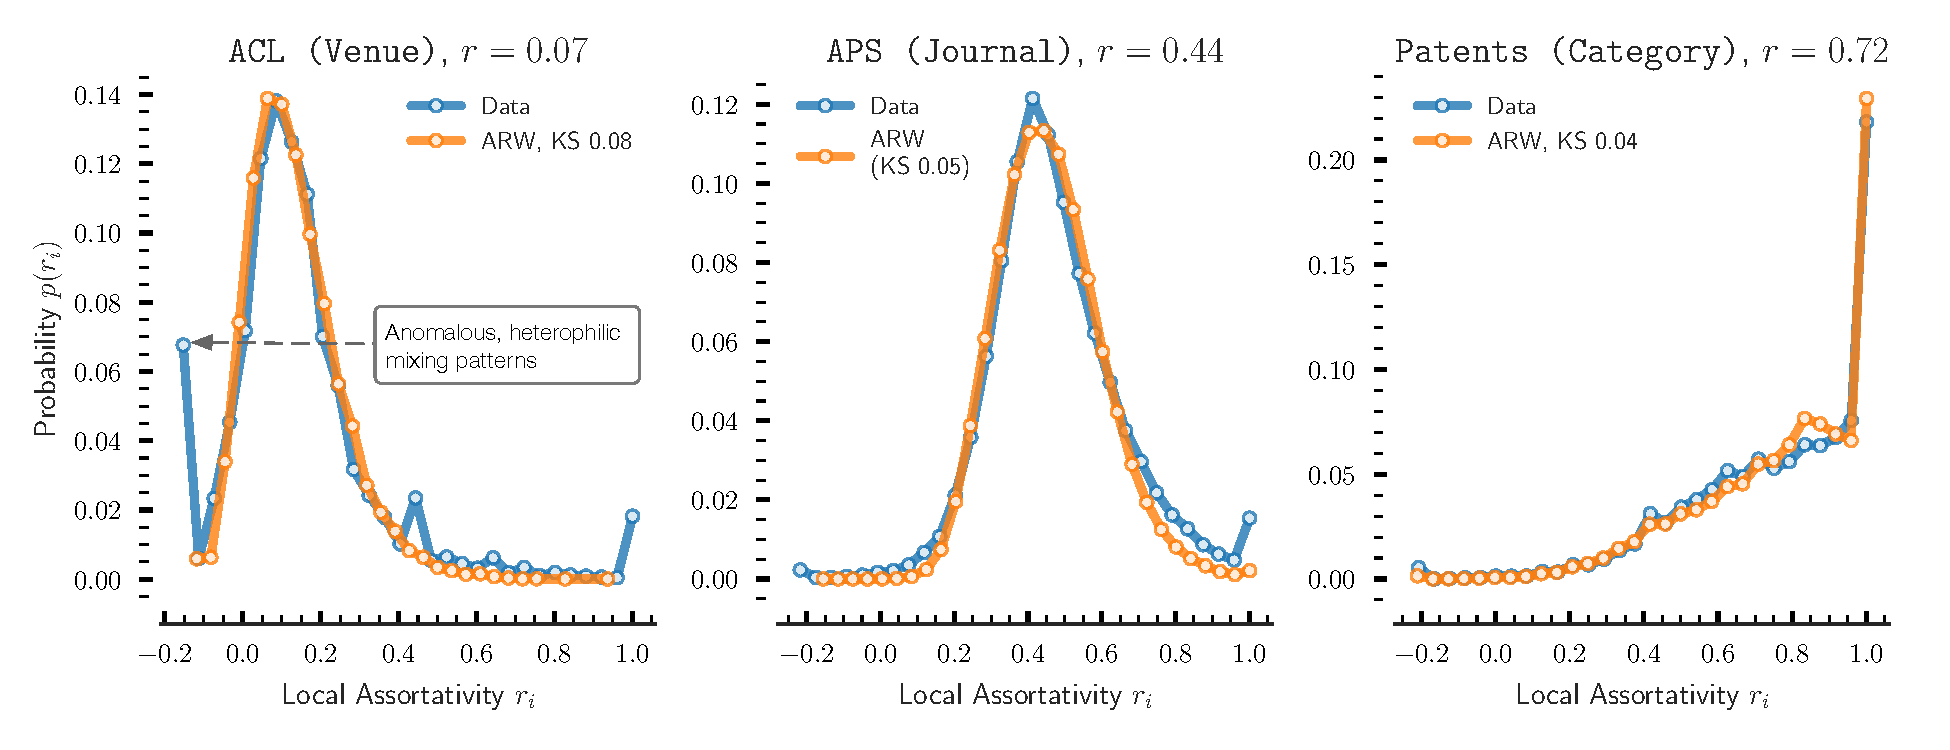
\includegraphics[width=\linewidth]{local_atty_dist}
    \caption{Local attribute mixing patterns of homophilic networks \texttt{ACL}, \texttt{APS}
    and \texttt{Patents} reveal anomalous, skewed and even heterophilic local mixing patterns.
    \texttt{ARW} preserves the observed local assortativity distributions with high accuracy,
    but does not account for nodes with extreme heterophilic or homophilic preferences.}
    \label{fig:local_atty}
\end{figure}
\texttt{ARW} can preserve
diverse local assortativity distributions with high accuracy even though nodes
share the same attribute preference parameter $p_a$. This is because  \texttt{ARW}
incorporates multiple sources of stochasticity through its edge formation
mechanism. As a result, incoming nodes with fixed homophilic preferences can end
up having variable local assortativity by (a) selecting a seed node in a region
with too few (or too many) similar nodes or (b) exhausting all its links before
visiting similar (or dissimilar) nodes.
However, \texttt{ARW} is not expressive enough to accurately model anomalous
mixing patterns. Richer mechanisms such as sampling $p_a$ from a mixture of
Bernoulli distributions are necessary to account for anomalous mixing patterns.

% The local assortativity coefficient $r_l(i)$ of node $i$,
% with outdegree $k(i)$ and attribute value $b(i)$, uses a distribution $w_i$ to
% reweigh edges based on how local they are to node $i$:
% \begin{equation*}
%     r_l(i) = \frac{\sum\limits_{b \in B} e_{bb}(i) - \sum\limits_{b \in B} e_{b.}e_{.b}}{1 - \sum\limits_{b \in B} e_{b.}e_{.b}}
% \end{equation*}


%
% Unlike global assortativity, local assortativity coefficient of node $i$,
% $r_l(i)$, compares the mixing patterns in node $i$'s locality to the expected
% mixing pattern if the edges were randomly rewired.
% Given a directed network $G=(V,E)$ with adjacency matrix $A$ and attribute
% values $B=\{b_1...b_m\}$, the local assortativity coefficient $r_l$ of node $i$
% with outdegree $k_i$ is defined as follows:
%


























% can generate network
% with tunable local clustering distribution and indegree-clustering relationship
% controls the effect of triadic closure using the jump parameter $p_j$ and link parameter
% $\alpha$. $p_j$ effectively incorporates structural constraints that limit the extent to
% which nodes explore the network whereas $\alpha$ indirectly controls the effect of
% triadic closure on edge formation.





% \subsection{Parameter space of \textsc{RW} model}
%
% Through a series of extensive experiments, we observe that our model \textsc{RW} is able
% to model multiple structural characteristics of real-world networks. However, the fitted
% parameters are different for each dataset, suggesting possibly different
% local growth mechanisms in each network.~\Cref{table:rw_parameters}
% describes the best fitted parameters for five citation networks used in
% our experiments.
%
%
% \begin{table}[!h]
% \center
% \caption{ Best fittedparameters obtained after grid search for random walk model. }
% \label{table:rw_parameters}
% \resizebox{\columnwidth}{!}{%
% \begin{tabular}{@{}cccccc@{}}
%  & \multicolumn{1}{c}{\textit{USSC}} & \multicolumn{1}{c}{\textit{HEP-PH}}& \multicolumn{1}{c}{\textit{APS}}& \multicolumn{1}{c}{\textit{Patents}} & \multicolumn{1}{c}{\textit{Semantic}} \\ \toprule
%  $p_l$ & 0.80 & 0.80 & 0.15 & 0.25 & 0.40 \\
%  $p_j$ & 0.30 & 0.65 & 0.65 & 0.05 & 0.15 \\
%  $p_o$ & 0.95 & 0.95 & 0.80 & 1.00 & 0.95 \\
%  $p_r$ & 0.50 & 0.80 & 0.85 & 0.45 & 0.60 \\ \midrule
% \end{tabular}
% }
% \end{table}

% To summarize, the experiment results on five citation networks against
% show that our resource-constrained model (\textsc{rw}) outperform four baseline
% growth models in accurately preserving degree, clustering and its relationship.

% Weighted relative error (\texttt{WRE})
% is used to measure the similarity between the indegree \& local clustering relationship in $G$ and $\hat{G}$:
% $$ \texttt{WRE}: \sum_{\text{Indeg.} k} P_{\textsc{g}}(k) \frac{c(k)-\hat{c}(k)}{c(k)} $$
% \texttt{WRE} is the weighted sum of the relative error between $c(k)$ and $\hat{c}(k)$,
% the average local clustering of nodes with degree $k$ in $G$ and $\hat{G}$ respectively;
% which aggregates the relative error between $c(k)$ and $\hat{c}(k)$,
% the average local clustering of nodes with degree $k$ in networks $G$
% and $\hat{G}$ respectively; The weight of each relative error term equals the probability
% mass $p_G(k)$ of indegree $k$ in the observed network $G$.

%
% \begin{figure*}
%  \centering
%  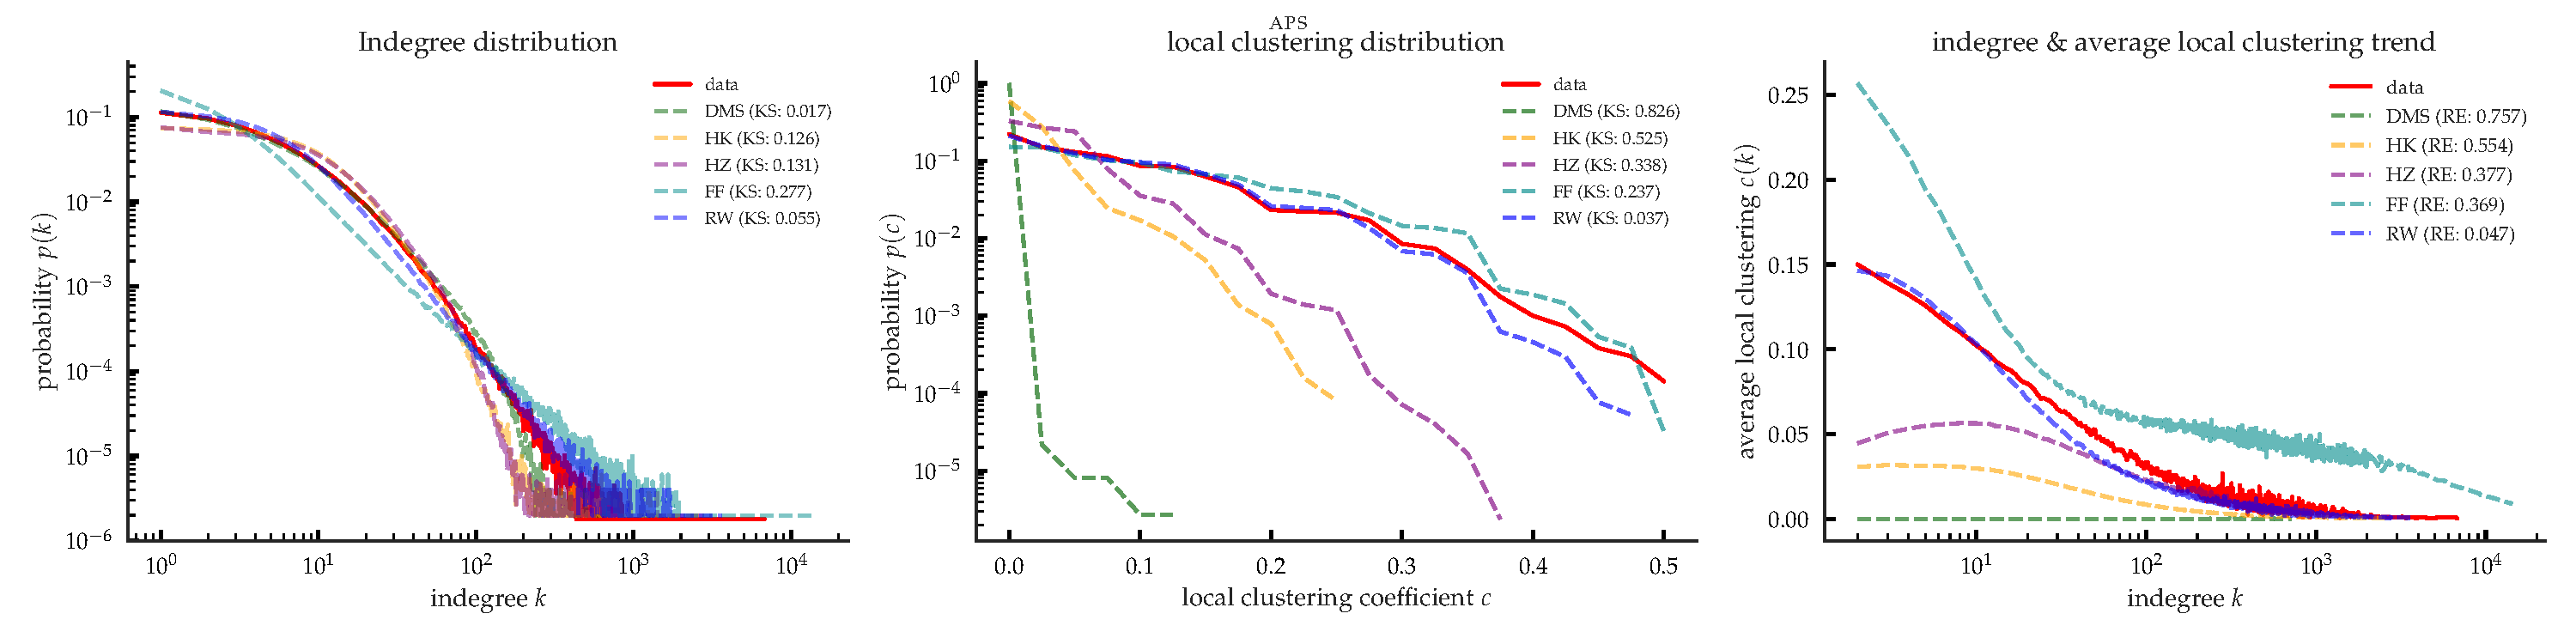
\includegraphics[width=\textwidth]{exp_aps}
%  \vspace{-12pt}
%
% \caption{Accuracy of growth models at preserving structural properties of \textsc{APS} network.
%  Our model \textsc{rw} outperforms the other in \textit{jointly} preserving heavy-tailed indegree
%  distribution, skewed local clustering distribution and the indegree \& average local clustering trend.}
%
% \label{fig:analysis}
% \end{figure*}
